
\startchapter{Proposed Approach}
\label{chapter:proposed}

Following the objective of the sections \ref{sec:nmf} and \ref{sec:repet}, I would like to narrow my focus to only one example that I believe has an obvious instrumental repetition, and I (and maybe others) have listened to it enough that can relate and interpret signals more effectively. Figure \ref{fig:billie-jean} shows the spectrum of the first 4 seconds of the song "Billie Jean" by Michael Jackson\cite{michael_jackson_billie_1982}. The song starts with 5 seconds of repeating drum hits before other instruments join and the singer starts singing after 25 seconds. This repeating drum continues for 4 minutes until the end of the song. So in this chapter, I am investigating if I can find a way to reuse this drum sound during the whole music and as a result, achieve an acceptable lossy audio compression.

\begin{figure}[ht]     
    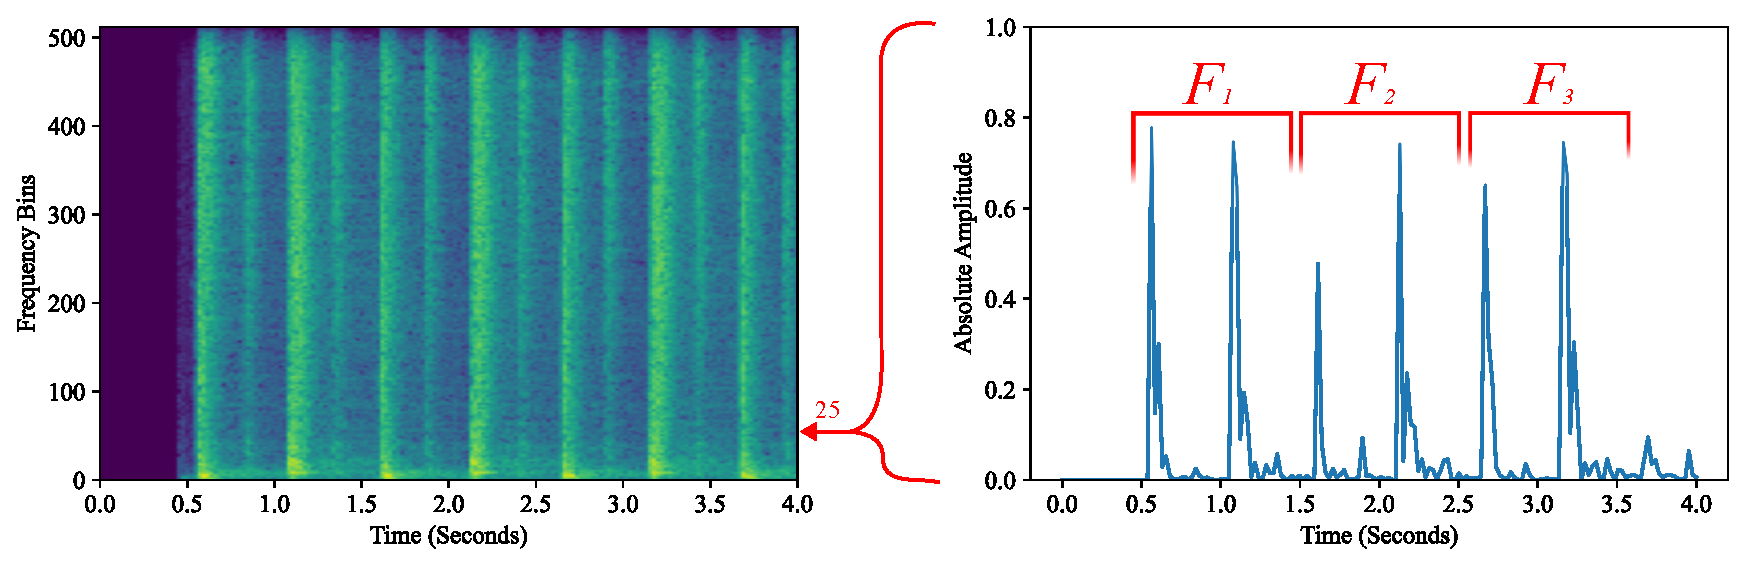
\includegraphics[width=\linewidth]{Figures/chap4/proposed/bj.eps}
    \caption{Illustration of repeating beats in the song "Billie Jean" by Michael Jackson\cite{michael_jackson_billie_1982} starting at the beginning.}
    \label{fig:billie-jean}
\end{figure}

\section{Main Idea}
\label{sec:idea}

To analyze the repeating signal easier, I focus on MDCT's 25th frequency bin which is shown on the right side of figure \ref{fig:billie-jean}. As can be seen in this Amplitude-Time plot, repeating drum sounds are visible as sudden spikes jumping from 0 to .8 in the amplitude. Knowing the song and seeing this plot, I can identify 3 repeating frames: first from 0.5 to 1.5 seconds ($F_1$), second from 1.5 to 2.5 seconds ($F_2$), and third from 2.5 to 3.5 seconds ($F_3$). As for a computer to identify matching frames, it can pick a frame (for example $F_3$) and loop through a shifting frame that is going backward in time while calculating the sum of absolute differences between these two frames. As can be seen in figure \ref{fig:shifting}, the output of this calculation has the minimum amount at 1 second. This means that the best candidate for $F_3$ to reuse is a frame starting 1 second earlier, i.e $F_2$.

\begin{figure}[ht] 
    \centering
    \includesvg[width=0.5\linewidth]{Figures/chap4/proposed/shift.svg}
    \caption{Sum of Absolute Differences between $F_3$ and a shifting frame going backwards in time.}
    \label{fig:shifting}
\end{figure}

The minimum amount in figure \ref{fig:shifting} is almost always not zero. That is because even though two audio signals sound identical to a human ear, they have some level of imperceptible differences. Figure \ref{fig:f3af2} shows these differences more clearly by overlapping both $F_3$ and $F_2$ on each other. When subtracting these two frames, as can be seen in figure \ref{fig:f3-f2}, the output is not zero, but it has some noises around the zero amplitude. This can be evidence of the reason the DEFLATE algorithm can not perform its lossless compression over songs with repeating tones because the repetition is not exact.

So because human ears can not perceive minor differences between $F_3$ and $F_2$, I propose that by manipulating signals we can help the DEFLATE algorithm and achieve a better compression size. This manipulation can be done by removing noises around the zero amplitude of differences between two frames using a threshold. Figure \ref{fig:f3-f2} shows this threshold should be able to separate perceptible differences from imperceptible ones. Applying this \textbf{Zero Threshold} would result in many zeros (figure \ref{fig:pframe3}) which can be useful for the DEFLATE algorithm to identify as a reusable signal. The resulting frame has similarities with P-Frames in the video encoding layer of MPEG-1 standard\cite{mpeg1-1993-video}.

\begin{figure}[ht]   
    \centering
    \begin{subfigure}{0.24\textwidth}
        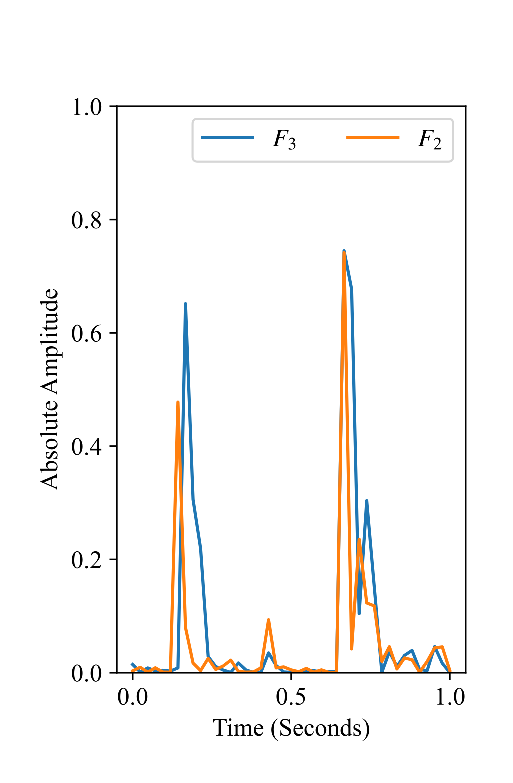
\includegraphics[width=\linewidth]{Figures/chap4/proposed/f3af2.eps}        
        \caption{$F_3$ and $F_2$}
        \label{fig:f3af2}
    \end{subfigure}
    \begin{subfigure}{0.24\textwidth}
        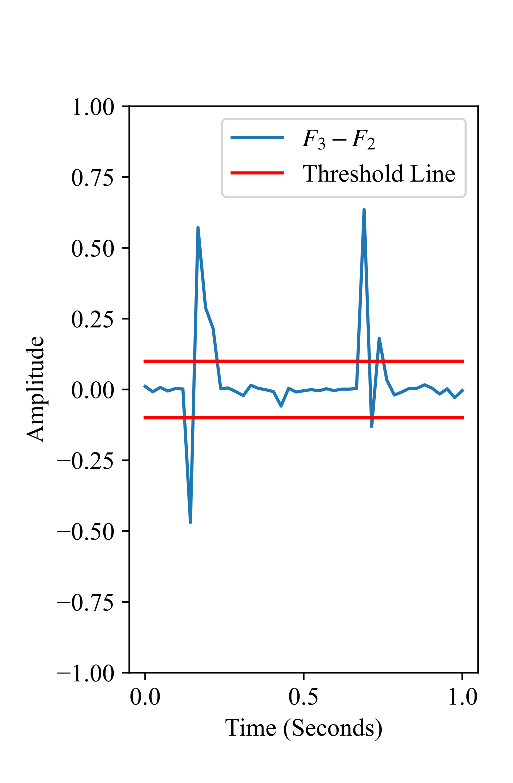
\includegraphics[width=\linewidth]{Figures/chap4/proposed/f3-f2.eps}        
        \caption{$F_3 - F_2$}
        \label{fig:f3-f2}
    \end{subfigure}
    \begin{subfigure}{0.24\textwidth}
        \includesvg[width=\linewidth]{Figures/chap4/proposed/pframe3.svg}
        \caption{$P_3$}
        \label{fig:pframe3}
    \end{subfigure}
    \begin{subfigure}{0.24\textwidth}
        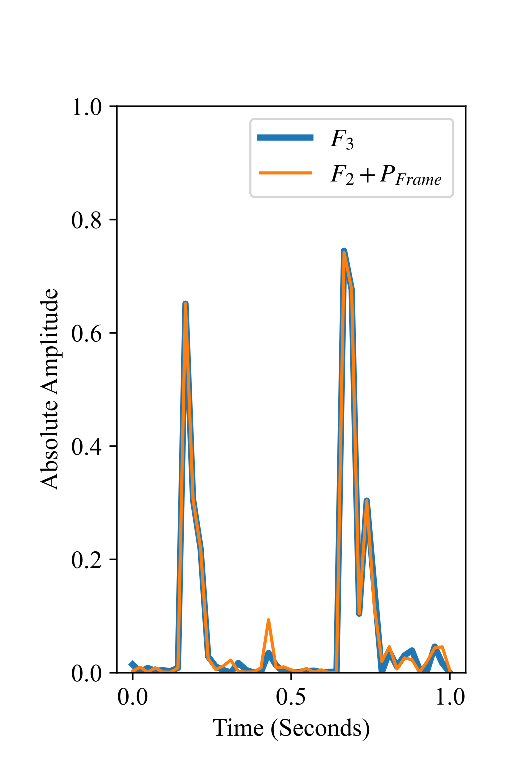
\includegraphics[width=\linewidth]{Figures/chap4/proposed/f3f2+p.eps}        
        \caption{$F_3$ and $F_2+P_3$}
        \label{fig:f3f2p}
    \end{subfigure}
    \caption{Illustration of P-Frame logic}
    \label{fig:pframe-logic}
\end{figure}

The rest of the properties of this audio compression idea are inspired by the MPEG-1 video encoder in which two types of frames are defined. \textbf{Intra-Frames or Independent-Frames (I-Frames)} are the ones that can be decoded independently and they contain a complete JPEG image. \textbf{Inter-Frames or Predicted-Frames (P-Frames)} are the ones that are dependent on another I-Frame or P-Frame to be decoded and they only contain the difference between the two images. 

So similar to the MPEG scheme, a frame that is made from the differences of audio frames can be named a P-Frame, while an independent audio frame can be named an I-Frame. The proposed encoding saves I-Frames alongside P-Frames. P-Frames also hold a number to indicate how many frames are they referring back in time while they are keeping only the differences between the frame at their place and the referred frame (as shown with arrows in figure \ref{fig:ipp}). The decoder would reconstruct frames by adding the referenced frame with the stored difference. Figure \ref{fig:f3f2p} shows the similarity of the original $F_3$ and the reconstructed signal. Obviously, the similarity between the original and the reconstructed signal is dependent on the threshold parameter. If the threshold parameter is chosen carelessly, it can produce perceptible differences in the decoded signal.

\begin{figure}[ht] 
    \centering
    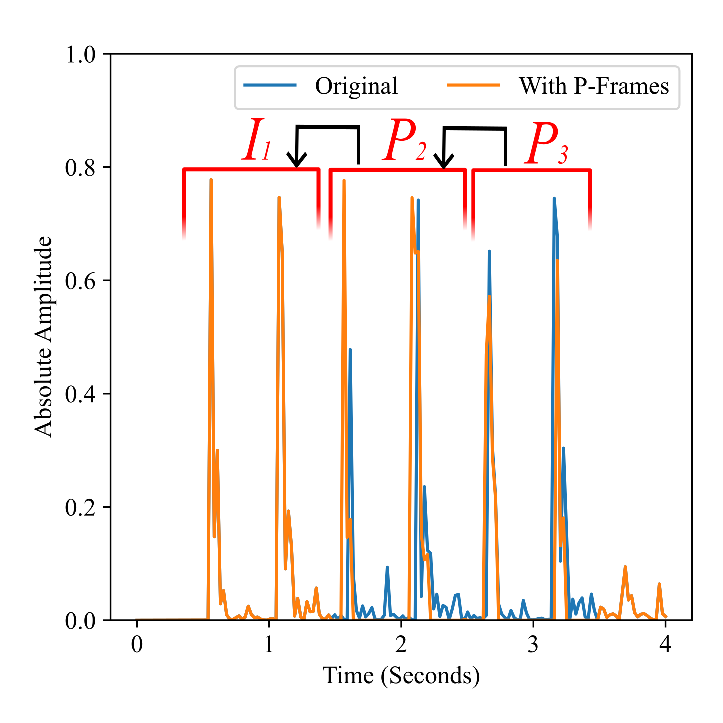
\includegraphics[width=0.5\linewidth, height=0.35\linewidth]{Figures/chap4/proposed/ipp.eps}
    \caption{Illustration of P-Frame logic and its comparison outcome with the original}
    \label{fig:ipp}
\end{figure}

To make this proposed approach more efficient, some conditions need to be defined and managed:
\begin{itemize}
    \item A P-Frame should be used only if it has less information compared to the corresponding I-Frame. In cases where a repeating frame can not be found, using a P-Frame would contain a greater or equal amount of information and therefore it would not useful for the compression size. 
    \item Each decoding from a P-Frame produces a signal that is imperceptible compared to the original. However, after continuous use of P-Frames, all these minor imperceptible differences can accumulate to some quiet but perceptible noises. Therefore, similar to the MPEG scheme, I-Frames should be forced to be used on a constant frequency. The frequency of I-Frame enforcement can be called \textbf{I-Rate}. 
    \item It would be very inefficient to find a suitable similarity between two frames that are 1 minute apart. Finding a suitable reference for a P-Frame should have a limit. Without this limit, the processing time would increase exponentially. We can use the same I-Rate parameter and enforce P-Frames not to look further behind an enforced I-Frame.
    \item It is not efficient for a frame to have the size of 1 second. Even though the 1 second was used in the example above for simpler analysis, in fact, a smaller frame size can increase the chances of finding similarities. I propose that we use one single MDCT time block (containing only 512 frequency bins) as a single frame.
\end{itemize}

\section{Implementation}
\label{sec:implementation}

Algorithm \ref{alg:find-pframe} shows a function that is responsible to find a suitable P-Frame using the conditions mentioned above. It creates an I-Frame as a comparison to all shifting P-Frames and chooses the one that would create the most number of zeros. The function then returns the generated frame ($F$) and the relative reference of a frame that was used to generate it ($r$). If the function decides on using an I-Frame, it would use zero inside the $r$ variable.

\begin{algorithm}[ht]
\caption{Finding the most similar frames for the encoding (P-Frame)}
\label{alg:find-pframe}
\begin{algorithmic}
\Function{EncodeFrame}{$M_{t\times 512}, t, iRate, iThreshold, pThreshold$}
    \State $P \gets$ \Call{Zeros}{$iRate$}
    \State $F \gets$ \Call{Zeros}{$iRate, 512$}
    \\
    \State $N \gets$ \Call{Max}{$M[t]$}
    \State $F[0] \gets$ \Call{Threshold}{$M[t], iThreshold \times N$} \Comment{The I-Frame}
    \State $P[0] \gets$ \Call{Count\_Zeros}{$F_0$}
    \\
    \For{$i=1$ \textbf{to} $iRate$}
        \If{($t - i) \mod{iRate} = 0$}
            \State \textbf{break} \Comment{The I-Rate Limit}
        \EndIf
        \\
        \State $dF \gets M[t] - M[t - i]$
        \State $F[i] \gets$ \Call{Threshold}{$dF, pThreshold$} \Comment{P-Frames}
        \State $P[i] \gets$ \Call{Count\_Zeros}{$F[i]$}
    \EndFor
    \\
    \State $r \gets$ \Call{ArgMax}{$P$} \Comment{Pick the Best}
    \State \Return $(r, F[r])$
\EndFunction
\end{algorithmic}
\end{algorithm}

As can be seen in algorithm \ref{alg:scheme}, by calling the defined function repeatedly over the whole MDCT matrix, we can achieve a modified matrix of frames and an array of all used references. These two data structures can then be given to the DEFLATE algorithm to store on a hard drive. Later for decoding, these two data structures can be reconstructed back from DEFLATE and P-Frames, identifiable by their non-zero reference, can be changed back into I-Frames by summing the referenced frame with the P-Frame. Lastly, the matrix can use the inverse of MDCT to produce raw audio signals.

\begin{algorithm}[ht]
\caption{Proposed new P-Frame scheme}\label{alg:scheme}
\begin{algorithmic}
\Function{Encode}{$W, iRate, iThreshold, pThreshold$}
    \State $M_{t \times 512} \gets \Call{MDCT}{W}$
    \State $R_t \gets$ \Call{Zeros}{$t$}
    \For{$i=0$ \textbf{to} $t$}
        \State $R[i], M[i] \gets$ \Call{EncodeFrame}{$M, i, iRate, iThreshold, pThreshold$}
    \EndFor
    \State \Return \Call{Deflate}{$R$}, \Call{Deflate}{$M$}
\EndFunction
\\
\Function{Decode}{$Z_r, Z_m$}    
    \State $M_{t \times b} \gets$ \Call{Deflate$^{-1}$}{$Z_m$}
    \State $R_{t} \gets$ \Call{Deflate$^{-1}$}{$Z_r$}
    \For{$i=0$ \textbf{to} $t$}
        \If{$R[i] > 0$}
            \State $M[i] \gets M[i] + M[i-R[i]]$
        \EndIf
    \EndFor
    \State \Return \Call{MDCT$^{-1}$}{$M$}
\EndFunction
\end{algorithmic}
\end{algorithm}

\section{Exploration Tests}
\label{sec:tests}

Now with the new P-Frame scheme defined, it is time to observe how it behaves on our chosen example, the "Billie Jean" song. The parameters that I used were: 2 seconds for I-Rate, $10^{-3}$ for P-Frame Threshold, and 0 for I-Frame Threshold. Looking at the histogram of generated references in figure \ref{fig:hist}, it can be seen that more than 98\% of frames were chosen to be P-Frames ($h(0)=1.5\%$) which means for each one of them, at least one element (2 bytes) became zero and helped to improve the compression. Interestingly, the histogram seems to be having jumps around 44 frames (1 second), 33 frames (.75 of a second), 22 frames (.5 of a second), and 11 frames (.25 of a second). This means that the algorithm is able to find the 1-second repeating beats and fractions of it based on the song's $4/4$ time signature. 

\begin{figure}[ht] 
    \centering
    \includesvg[width=0.5\linewidth]{Figures/chap4/tests/hist.svg}
    \caption{Histogram of References from P-Frame encoding over the song "Billie Jean" by Michael Jackson}
    \label{fig:hist}
\end{figure}

Most noticeably in Figure \ref{fig:hist}, we can see that more than 13.2\% of P-Frames refer to their most immediate previous frame ($\sim .023$ of a second) and more than 5\% refer to their second most immediate previous frame ($\sim .045$ of a second). This probably means even though repeating beats and notes can have similar frames, those frames related to the same tone are even more similar. Looking at the differences between I-Frame only and P-Frame spectrum in figure \ref{fig:billie_jean_25sec}, we can see that \ref{fig:saved_25sec} has darker areas where the red line is higher as compared to the \ref{fig:unmodified_25sec}, especially in areas that the drum sound is fading. This is an indication of saved bytes by reusing previous information in every P-Frame.

Looking at the used references in Figure \ref{fig:ref_25sec}, we can see that between 0 to 2 seconds, the distance of references increases linearly except for areas where an unfamiliar or new signal is played. At 2 seconds, because the parameter I-Rate was set, references suddenly drop to zero and they would not refer to any frames before 2 seconds. This will be repeated every 2 seconds.

\begin{figure}[ht]
\centering
\begin{subfigure}{0.30\textwidth}
    \includesvg[width=\linewidth]{Figures/chap4/tests/billie_jean_2.5sec.svg}
    \caption{I-Frames Only}
    \label{fig:unmodified_25sec}
\end{subfigure}
\hfill
\begin{subfigure}{0.32\textwidth}
    \includesvg[width=\linewidth]{Figures/chap4/tests/saved_2.5sec.svg}
    \caption{P-Frames \& Saved Bytes}
    \label{fig:saved_25sec}
\end{subfigure}
\hfill
\begin{subfigure}{0.32\textwidth}
    \includesvg[width=\linewidth]{Figures/chap4/tests/ref_2.5sec.svg}
    \caption{P-Frames \& References}
    \label{fig:ref_25sec}
\end{subfigure}
\caption{Effectiveness of IP-Frames over the drums in the beginning song "Billie Jean" by Michael Jackson}
\label{fig:billie_jean_25sec}
\end{figure}

In a different part of the song where more musical instruments are being played and Michael Jackson starts singing, we can see in figure \ref{fig:saved_3sec} shows fewer saved bytes as compared to \ref{fig:unmodified_3sec}. Expectedly, at 29.5 seconds where vocal signals seem to look more chaotic and less repetitive, we can see that the algorithm has failed to find similarities with previous frames. Similarly, in figure \ref{fig:ref_3sec}, we can see that the distance of references suddenly drops at 29.5 seconds before I-Rate enforces an I-Frame at 30 seconds. This would be an indication that the IP-Frame schema behaves differently in different parts of music depending on its ability to detect and reuse similar or repeated information.

\begin{figure}[ht]
\centering
\begin{subfigure}{0.30\textwidth}
    \includesvg[width=\linewidth]{Figures/chap4/tests/billie_jean_3sec.svg}
    \caption{I-Frames Only}
    \label{fig:unmodified_3sec}
\end{subfigure}
\hfill
\begin{subfigure}{0.32\textwidth}
    \includesvg[width=\linewidth]{Figures/chap4/tests/saved_3sec.svg}
    \caption{P-Frames \& Saved Bytes}
    \label{fig:saved_3sec}
\end{subfigure}
\hfill
\begin{subfigure}{0.32\textwidth}
    \includesvg[width=\linewidth]{Figures/chap4/tests/ref_3sec.svg}
    \caption{P-Frames \& References}
    \label{fig:ref_3sec}
\end{subfigure}
\caption{Effectiveness of IP-Frames over the vocals in the song "Billie Jean" by Michael Jackson}
\label{fig:billie_jean_3sec}
\end{figure}

Overall, with the specified parameters, the P-Frame encoder is able to compress the "Billie Jean" song by more than 89.5 \% as compared to the lossless I-Frame scheme which is 95.1 \%. Because no other perceptual techniques were active, this means the P-Frame scheme alone has a 5.6 \% improvement in compression ratio. Evaluating the perceptual audio quality of the decoded signal, I got -.858 for the objective difference degree which means the difference between the original and the decoded signal is hard to perceive by the human ears.

The aforementioned results for this specific example indicate that the new approach is feasible and does a good job of compressing "Billie Jean"  song. Moreover, more songs are required to be tested and analyzed in order to consider these results more generally applicable. To investigate this, I run the P-Frame scheme on a larger dataset and I analyze these results statistically in chapter \ref{chapter:Exp}.